\documentclass[12pt,a4paper]{scrartcl}
\usepackage[utf8x]{inputenc}
\usepackage{ucs}
\usepackage{amsmath}
\usepackage{amsfonts}
\usepackage{amssymb}

\usepackage{subfigure}
\usepackage{graphicx}

\newcommand{\e}[1]{\ensuremath{\times 10^{#1}}}

\parskip1.5ex plus1ex minus0.5ex

\author{Simon Wallner}
\title{Implementation of Rea1l Time Atmospheric Scattering}


\begin{document}
\maketitle


\begin{abstract}
This document accompanies a small demo implementation of \cite{HoffmanPreetham02Rendering-outdoor}'s atmospheric scattering model. The Implementation tries to follow the paper closely but diverges in some aspects. Below you will find more detail on the general approach, the divergences and where the results differ from the original implementation.
\end{abstract}


\section{Background}
The atmospheric scattering model \cite{HoffmanPreetham02Rendering-outdoor} was released in 2002 and more information about this approach can also be found in \cite{03ATI-LightScattering} and \cite{Preetham03Modeling-skylight}. Earlier relevant work for this approach is \cite{PreethamShirleySmits99A-practical-analytic}.

The model uses Rayleigh and Mie scattering to model scattering in the earth's atmosphere. A few simplifications are made to make the model work in real time on current and even last generation consumer hardware.


\section{Model and Simplifications}
The model only accounts for single scattering events, and constant density mediums. Earth's curvature is only taken account in and approximated in the skylight computation. In the case of aerial perspective earth is assumed to be flat.

\section{Implementation}
The demo was implemented with the information found in the above mentioned papers. It is implemented as a OpenGL demo 3.2, with GLSL shaders. Most of the implementation is done in the fragment shader, although big parts could have been offloaded to the vertex engine for similar results (dependent on scene tessellation).

computations are done HDR and a simple log-luminance centred linear tone mapping operator is used as a post process to display the image.

\subsection{General}
Atmospheric scattering is highly wavelength dependent, and therefore computations are performed for 3 selected wavelengths. This solution is by no means correct but gives a good looking approximation. The three used primaries are (according to \cite{03ATI-LightScattering}) 400nm, 530nm and 700nm. 

\subsection{Divergences}
The implementation diverges from the papers in a few aspects. The scale factor for the Rayleigh phase function was chosen differently to achieve better looking results. 

The \emph{concentration factor} used in the Mie scattering function was computed differently as the formula in \cite{PreethamShirleySmits99A-practical-analytic} did not match the numbers in \cite{03ATI-LightScattering}.



\subsection{Skylight}
the curvature of the earth's surface is approximated with by the function given in \cite{03ATI-LightScattering}
\begin{equation}
\frac{l(\theta_s)}{l_{zenith}} = \frac{1}{\cos \theta_s + 0.15(93.885 - \theta_s)^{-1.253}}
\end{equation}

where $\theta_s$ is the zenith angle and $l_zenith$ is the optical length of the medium in zenith direction. In the paper these lengths are given as $8.4km$ for molecules (Rayleigh scatterers) and $1.25km$ for aerosols (Mie scatterers).

the above formula is only usefull in the range of $[0, 90]$ degrees and is therefore capped, even though zenith angles of wenn above $90\deg$ can occur. 

The sky is generally assumed to be black (except for a faint skymap) and sky color is only a result of in-scattering. 

To approximate the earth shadow a very crude approximation is used. The sun light's intensity is attenuated as the sun approaches the horizon. 



\subsection{Aerial Perspective}
For aerial perspective the incident light on the ground is first computed by calculating extinction and in-scattering in the direction of the sun. 

This incident light is then used to shade the ground and is then attenuated by the out-scattering as it travels towards the viewer. Atmosphere is assumed to be of constant density at ground level which simplifies computations. In-scattering is also evaluated and added to the result.



\section{Results and Discussion}
Although most parts are implemented in the fragment shader, rendering takes only about 10ms per frame on standard consumer hardware\footnote{ATI Radeon 4830} at a resolution of $1280 \times 720$. 

The Result looks pleasing and lifelike for most parameter choices. A big difference however is in situations where the sun is close to the horizon. The typical yellow-reddish sky of the rising and setting sun could not be achieved with the present implementation. 

However, this effect can be clearly seen in the reference demo provided by Preetham and Hoffman. I assume that either my implementation is fundamentally flawed or not all implementation details are revealed in the cited papers.

\begin{figure}[hbtp]
\centering
\subfigure[reference]{
	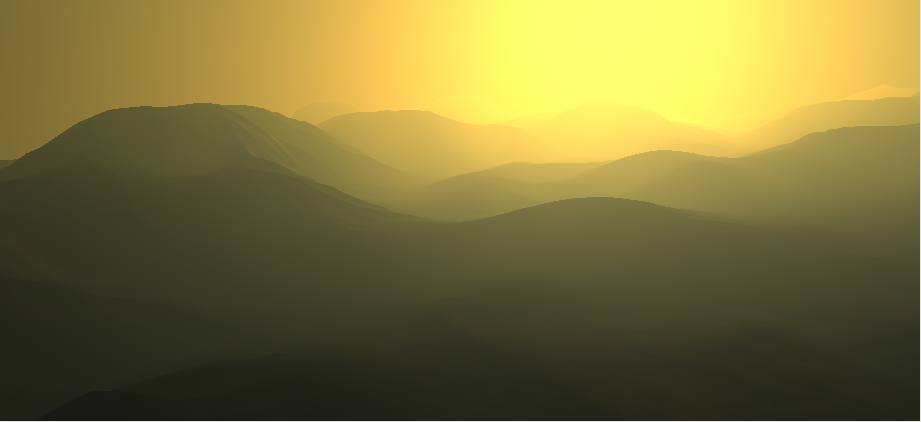
\includegraphics[width=0.45\columnwidth]{img/sunset-reference}
}
\subfigure[result]{
	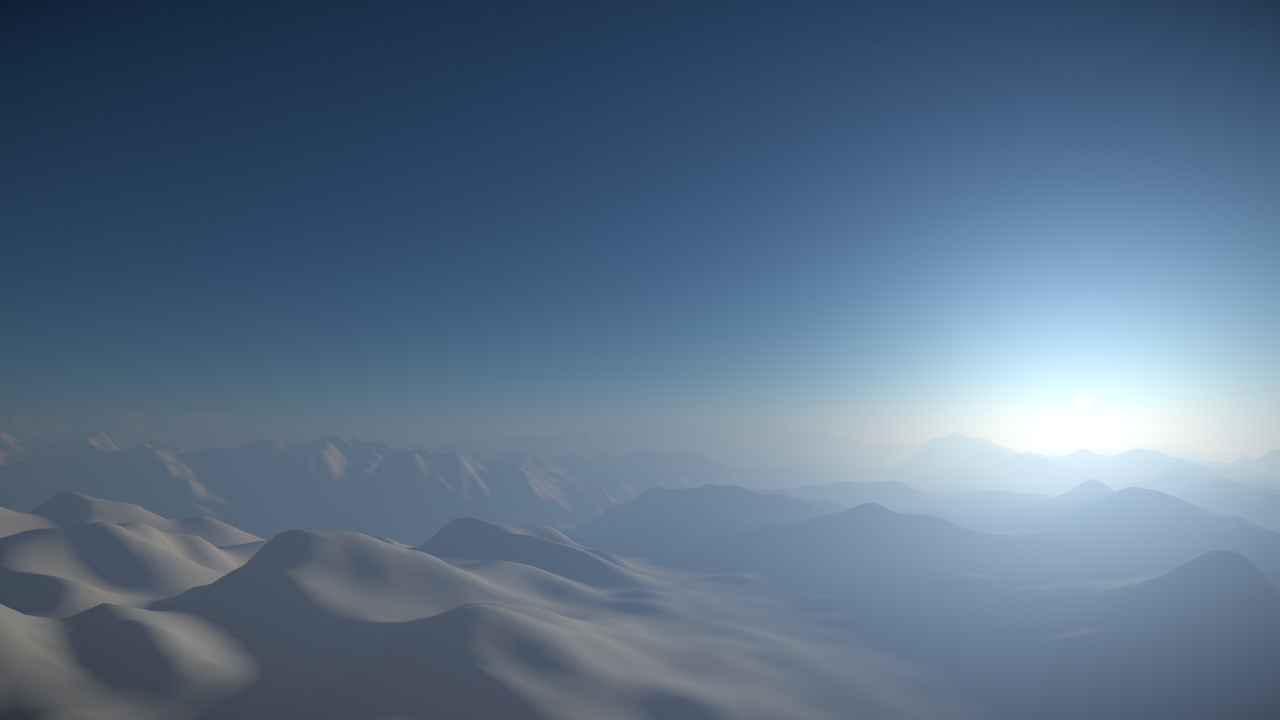
\includegraphics[width=0.45\columnwidth]{img/sunset}
}

\end{figure}




\bibliographystyle{apalike}
\bibliography{literature}
\end{document}